\documentclass[a4paper]{article}
\usepackage{amsmath}
\usepackage{pythonhighlight}
\usepackage{graphicx}

\title{Statistical Modelling\\
Coursework 2}
\author{Stefan A. Obada - \textit{so1118}}
\date{March 2020}
\makeindex
\setcounter{secnumdepth}{0} % sections are level 1

\begin{document}

\maketitle

\begin{abstract}
	This paper solves the second Coursework available on Blackboard. Check (\footnote{https://github.com/stefan-obada/csw-stats-2}) for full documentation.
\end{abstract}

\tableofcontents



\newpage

\section{Question 1}

\subsection{a)}
As we are working under $(FR)$ and $(SOA)$ we can solve for $\hat{\gamma}_{LSE}$ as: $\hat{\gamma}_{LSE} = (X^{T}X)^{-1}X^{T}\textbf{Y}$, where $X$ is the design matrix. In our case:
\begin{equation*}
X = 
	\begin{bmatrix}
	1 & w_{1} & x_{1} \\
	1 & w_{2} & x_{2} \\
	\vdots  & \vdots  & \vdots \\
	1 & w_{n} & x_{n} 
	\end{bmatrix}
\end{equation*}

\begin{equation*}
X^{T}X = 
	\begin{bmatrix}
	n & n\overline{w} & n\overline{x} \\
	n\overline{w} & \sum{w_{i}^2} & \sum{w_{i}x_{i}} \\
	n\overline{x} & \sum{w_{i}x_{i}} & \sum{x_{i}^2}
	\end{bmatrix}
\end{equation*}

Using the following 2 properties for the 3x3 matrix inverse and for $S_{ab}$ we will deduce the form of $(X^{T}X)^{-1}$ and $X^{T}\textbf{Y}$. We will skip the matrix calculation part.
\vspace{2.5mm}
\hrule
\begin{equation}
\begin{split}
\left(\begin{array}{ccc}
a&b&c\\
d&e&f\\
g&h&i
\end{array}\right)^{-1}
=&
{1 \over {\rm{det()}}}
\left(\begin{array}{rrr}
e i - f h&-(b i - c h)&b f - c e\\
-(d i - f g)&a i - c g&-(a f -c d)\\
d h - e g&-(a h - b g)&a e - b d
\end{array}\right)\\
=&
{1 \over {\rm{det()}}}
\left(\begin{array}{rrr}
a' & b' & c'\\
d' & e' & f'\\
g' & h' & i'
\end{array}\right)
\end{split}
\end{equation}

\begin{equation}
\begin{split}
& S_{ab} = \sum_{i}{(a_{i}-\overline{a})(b_{i}-\overline{b})} = \sum{(a_{i}b_{i} - a_{i}\overline{b}-\overline{a}b_{i} + \overline{a}\overline{b})} = \\ 
& \sum{a_{i}b_{i}} - 2n\overline{a}\overline{b} + n\overline{a}\overline{b} = \sum{a_{i}b_{i}} - n\overline{a}\overline{b}. \\ 
& Moreover: S_{aa} = \sum{a_{i}^2} - n\overline{a}^2
\end{split}
\end{equation}
\hrule
\vspace{2.5mm}
Therefore, we deduce:
\begin{equation*}
(X^{T}X)^{-1} = \frac{1}{n(S_{xx}S_{ww}-S_{xw}^2)}
	\begin{bmatrix}
	a' & b' & c'\\
	d' & e' & f'\\
	g' & h' & i'
	\end{bmatrix}
\end{equation*}

\begin{equation*}
X^{T}\textbf{Y} = 
	\begin{bmatrix}
	\overline{Y} \\
	S_{wy} + n\overline{w}\overline{Y} \\
	S_{xy} + n\overline{x}\overline{Y}
	\end{bmatrix} 
\end{equation*}

\begin{equation*}
(X^{T}X)^{-1}X^{T}\textbf{Y} = 
	\frac{1}{n(S_{xx}S_{ww}-S_{xw}^2)}
	\begin{bmatrix}
	a'\overline{Y} + b'(S_{wy} + n\overline{w}\overline{Y}) + c'(S_{xy} + n\overline{x}\overline{Y}) \\
	d'\overline{Y} + e'(S_{wy} + n\overline{w}\overline{Y}) + f'(S_{xy} + n\overline{x}\overline{Y}) \\
	g'\overline{Y} + h'(S_{wy} + n\overline{w}\overline{Y}) + i'(S_{xy} + n\overline{x}\overline{Y}) \\
	\end{bmatrix} 
\end{equation*}
Now plugging the values for $(a', b' ... i')$ and rearranging \textbf{(see Appendix 1)} we find:

\begin{equation*}
\begin{split}
\hat{\gamma}_{LSE} = & (X^{T}X)^{-1}X^{T}\textbf{Y} = \\
	= & \frac{1}{(S_{xx}S_{ww}-S_{xw}^2)}
	\begin{bmatrix}
	(S_{ww}S_{wx}-S_{xw}^2)\overline{Y} - \overline{w}(S_{wy}S_{xx} - S_{wx}S_{xy}) - \overline{x}(S_{xy}S_{ww} - S_{wx}S_{xy}) \\
	S_{wy}S_{xx} - S_{wx}S_{xy} \\
	S_{xy}S_{ww} - S_{wx}S_{wy} \\
	\end{bmatrix} 
\end{split}
\end{equation*}
Therefore, we obtain the final estimators as:
\begin{equation*}
\begin{split}
	\hat{\gamma}_{0} = & \overline{Y} - \overline{w}\hat{\gamma}_{W} - \overline{x}\hat{\gamma}_{X} \\
	\hat{\gamma}_{W} = & \frac{S_{wy}S_{xx} - S_{wx}S_{xy}}{S_{xx}S_{ww}-S_{xw}^2} \\
	\hat{\gamma}_{X} = & \frac{S_{xy}S_{ww} - S_{wx}S_{wy}}{S_{xx}S_{ww}-S_{xw}^2} \\
\end{split}
\end{equation*}

\subsection{b)}

As proved in lectures, we have the following formula for $\hat{\beta}_{X}$:
\begin{equation*}
	\hat{\beta}_{X} = \frac{S_{xy}}{S_{xx}}
\end{equation*}
Therefore after factorization we can condition on $\textbf{x}-\overline{\textbf{x}}$ and $\textbf{w}-\overline{\textbf{w}}$ as it follows:
\begin{equation*}
\begin{split}
	\hat{\beta}_{X} = \hat{\gamma}_{X} \Leftrightarrow & \frac{S_{xy}S_{ww} - S_{wx}S_{wy}}{S_{xx}S_{ww}-S_{xw}^2} = \frac{S_{xy}}{S_{xx}}  \Leftrightarrow (case \; S_{xy}\neq0) \\
	\Leftrightarrow & S_{xx}S_{xy}S_{ww}-S_{xx}S_{wx}S_{wy} = S_{xy}S_{xx}S_{ww} - S_{xw}^2S_{xy} \Leftrightarrow \\
	\Leftrightarrow & S_{xx}S_{wy}=S_{wx}S_{xy} \; or \; S_{xw}=0 \\
\end{split}
\end{equation*}
\textbf{Case 1:} $S_{xx}S_{wy}=S_{wx}S_{xy}$ and $S_{xy}\neq0$ $\Rightarrow \hat{\gamma}_{W}=0$, which is trivial since it would reduce the second model to the first.\\
\textbf{Case 2:} $S_{xy} = 0 \Rightarrow \hat{\beta}_{X}=0 \Rightarrow \hat{\gamma}_{X}=0$, which is trivial again.  \\
\textbf{Case 3:} $S_{xw} = 0$ and $S_{xy}\neq0$, which is possible.

\subsection{c)}
Again, as proved in lectures we have:
\begin{equation*}
\begin{split}
	cov(\hat{\beta}_{X}) & = \frac{\sigma^2}{S_{xx}}\\
	cov(\hat{\gamma}_{LSE}) & = \sigma^2(X^TX)^{-1} \Rightarrow cov(\hat{\gamma}_{X}) = \frac{\sigma^2i'}{n(S_{xx}S_{ww}-S_{xw}^2)} = \\
	& = \frac{n\sigma^2S_{ww}}{n(S_{xx}S_{ww}-S_{xw}^2)} = \frac{\sigma^2}{S_{xx}-{S_{xw}^2}/{S_{ww}}} \\
	& = \frac{\sigma^2}{S_{xx}} \cdot (1-\frac{S_{xw}^2}{S_{xx}S_{ww}})^{-1} \\
\end{split}
\end{equation*}
\begin{itemize}
	\item Under the condition from \textbf{1b)} we have that $S_{xw}=0$ and therefore they will be equal.
	\item $\underline{var(\hat{\gamma}_{X})<var(\hat{\beta}_{X})} \Leftrightarrow (1-\frac{S_{xw}^2}{S_{xx}S_{ww}})^{-1}<1 \Leftrightarrow 1-\frac{S_{xw}^2}{S_{xx}S_{ww}} < 0 \Leftrightarrow \\ \Leftrightarrow \underline{S_{xw}^2>S_{xx}S_{ww}}$ (since otherwise $\frac{S_{xw}^2}{S_{xx}S_{ww}}<0$ but $S_{aa}>0$). However this cannot ever happen since by letting $\textbf{u}=\textbf{x}-\overline{\textbf{x}}$ and $\textbf{v}=\textbf{w}-\overline{\textbf{w}}$, the last relation is therefore equivalent to: $\langle\textbf{u}, \textbf{v}\rangle\langle\textbf{u}, \textbf{v}\rangle > \langle\textbf{u}, \textbf{u}\rangle\langle\textbf{v}, \textbf{v}\rangle$ which contradicts Cauchy–Bunyakovsky–Schwarz inequality.
	\item $\underline{var(\hat{\gamma}_{X})>var(\hat{\beta}_{X})} \Leftrightarrow \underline{S_{xw}^2<S_{xx}S_{ww}}$ by a similar argument. This explains that by adding a new parameter in a linear model results in an increased variance of the initial parameters.
\end{itemize}

\section{Question 2}
Through the solution code I use the following header, where we import the data and define \textit{LinearRegression} class which simply fits the Least Squares Estimator.
\begin{python}
	import pandas as pd
	import numpy as np
	import matplotlib.pyplot as plt
	
	## Import data
	df = pd.read_csv('fev.csv')
	X = df[['smoke', 'age']]
	y = df['fev'].values.reshape(-1,1)
	
	## Linear regression fit
	class LinearRegression():
	    """Simple LSE computing for Linear Regression"""
	    
	    @staticmethod
	    def append_ones(X):
	        # Appends a column of ones to X
	        X = np.concatenate([np.ones(shape=(X.shape[0], 1)), X], axis=1)
	        return X
	    
	    def fit(self, X, y):
	        X = self.append_ones(X)
	        # Least Squares method
	        LSE = np.linalg.inv(X.T.dot(X)).dot(X.T).dot(y)
	        self.intercept = LSE[0]
	        self.coef = LSE[1:]
\end{python}
\subsection{a)}
To compute the least squares estimators we will use the LinearRegression(). It simply calculates the least squares estimators as $(X^{T}X)^{-1}X^{T}\textbf{Y}$, also handling automatically adding the columns of ones to the design matrix. $\hat{\beta}_0$ and $\hat{\beta}_1$ will therefore be the \textit{intercept} and the \textit{coef} of the model.
\begin{python}
	# 2 (a) #
	X_fev = df.smoke.values.reshape(-1,1) # Design matrix with only smoke as covariate
	
	## Build the model
	model = LinearRegression() # Instance of the class
	
	## Fit the model
	model.fit(X_fev, y)
	
	#beta0 is the intercept and beta1 is the coef
	beta0 = model.intercept
	beta1 = model.coef[0]
	print(f'beta0 = {beta0}')
	print(f'beta1 = {beta1}')
\end{python}
\textbf{Output:}
\begin{python}
	beta0 = 3.9875804623220583
	beta1 = -0.71071892386052
\end{python}
Moreover, we can compute $E(fev|smoke=1)-E(fev|smoke=2)$ as:
\begin{python}
	## Mean difference
	exp_diff = (beta0 + 1*beta1) - (beta0 + 2*beta1)
	print('Fev(smokers) - Fev(nonsmokers): {}'.format(exp_diff))
	##
\end{python}
\textbf{Output:}
\begin{python}
	Fev(smokers) - Fev(nonsmokers): 0.71071892386052
\end{python}
\textbf{Conclusion:}
According to the estimates, smoking does not seem to impair lung function in children and it even contradicts the initial hypothesis that FEV is should be smaller for smokers. However, we will see that this result is not credible and we have to take into account another covariate: \textit{age}. Explore in \textbf{Appendix 2} more about this.

\subsection{b)}
Proceeding similarly as before, we will use \textit{LinearRegression()}.
\begin{python}
	# 2 (b)
	# Recall that X = df[['smoke', 'age']]
	
	## Fitting the model
	model_b = LinearRegression()
	model_b.fit(X, y)
	
	gamma0, gamma1, gamma2 = model_b.intercept, model_b.coef[0], model_b.coef[1]
	print(f'gamma0 = {gamma0}')
	print(f'gamma1 = {gamma1}')
	print(f'gamma2 = {gamma2}')
	##
\end{python}
\textbf{Output:}
\begin{python}
	gamma0 = -0.05061671981585736
	gamma1 = 0.20899487720480997
	gamma2 = 0.2306045731168579
\end{python}
And the mean difference:
\begin{python}
	## Mean difference
	exp_diff = gamma1*1-gamma1*2
	print('Fev(smokers) - Fev(nonsmokers): {}'.format(exp_diff))
	##
\end{python}
\textbf{Output:}
\begin{python}
	Fev(smokers) - Fev(nonsmokers): -0.20899487720480997
\end{python}
\textbf{Conclusion:} This results are indeed more realistic and shows that among children, smokers tend to have a \textit{0.2} decrease in FEV compared to non-smokers.\\
\\
Moreover, according to \textbf{1c)} we should have $\frac{var(\hat{\beta}_{1})}{var(\hat{\gamma}_{1})}<1$. We compute it with the previous formulae: $\frac{var(\hat{\beta}_{1})}{var(\hat{\gamma}_{1})} = 1-\frac{S_{xw}^2}{S_{xx}S_{ww}}$.

\begin{python}
	## Variability
	def S(a: np.array, b: np.array):
	    '''Return S_{ab} as in the coursework'''
	    return (a-a.mean()).dot(b-b.mean())
	
	print('var(beta1)/var(gamma1) = {}'.format((1-S(X.smoke,X.age)**2/(S(X.smoke,X.smoke)*S(X.age, X.age)))))
\end{python}
\textbf{Output:}
\begin{python}
	var(beta1)/var(gamma1) = 0.8365799359665773
	# Which is smaller than 1 and 
	# the variability in the new model is higher.
\end{python}

\subsection{c)}
Using \textit{Lemma 26} from the lecture notes with $\textbf{c}=\begin{bmatrix}0\\1\end{bmatrix}$ we can construct a $(1-\alpha)$ CI for $\beta_{1}$ as it follows:
\begin{equation*}
\frac{\hat{\beta}_{1}-\beta_{1}}{\sqrt{[(X^TX)^{-1}]_{2,2}\frac{RSS}{n-p}}} \sim t_{n-p} \Rightarrow
\end{equation*}
\begin{equation*}
\frac{\hat{\beta}_{1}-\beta_{1}}{\sqrt{\frac{n}{n\sum{smoke_{i}^2}-n^2(\overline{smoke})^2}\frac{RSS}{n-p}}} \sim t_{n-p} \Rightarrow
\end{equation*}
\begin{equation*}
I = ( \; \hat{\beta}_{1} \pm t_{n-p,\frac{\alpha}{2}} \cdot \sqrt{\frac{n}{n\sum{smoke_{i}^2}-n^2(\overline{smoke})^2}\frac{RSS}{n-p}} \; )
\end{equation*}
\begin{python}
	## 2c)
	alfa=0.05
	n = X_a.shape[0]
	
	# Build the full design matrix
	X_a_with_ones = LinearRegression.append_ones(X_a)
	# Compute RSS
	RSS = np.linalg.norm(y-X_a_with_ones.dot(np.array([beta0, beta1])))
	import scipy.stats # For t-distribution
	t_dist = scipy.stats.t
	# Compute the "inverse CDF"
	t_alfa = t_dist.ppf(1-alfa/2, df=n-2) 
	
	sum_smoke_squared = sum(X_a**2) # Sum(smoke_i^2)
	# Computer lower and upper part of interval
	lower = beta1-t_alfa*np.sqrt(n*RSS/(n*sum_smoke_squared-(n**2)*((X_a.mean())**2))/(n-2))
	upper = beta1+t_alfa*np.sqrt(n*RSS/(n*sum_smoke_squared-(n**2)*((X_a.mean())**2))/(n-2))
	print('A {}% CI for beta1 is: ( {:.3}, {:.3} )'.format((1-alfa)*100, lower[0], upper[0]))
	##
\end{python}
\begin{python}
	A 95.0% CI for beta1 is: ( -0.927, -0.495 )
\end{python}
Moreover we will construct the following hypothesis $\alpha$-level F-test \underline{$H_{0}:\beta_{1}=0$}, which is equivalent to $H_{0}: \textbf{Y} \in span(\begin{bmatrix} 1 \\ \vdots \\ 1 \end{bmatrix})$. We reject if $F=\frac{RSS_{0}-RSS}{RSS}\cdot\frac{n-r}{r-s}>c$ where $c$ is such that $P(F_{r-s,n-r} \geq c)=\alpha$. \\
\begin{python}
	## F_test 2c)
	alfa=0.05
	n = X_a.shape[0]
	r = 2
	s = 1
	X_a_without_smoke = np.ones(n) # Design matrix without the smoke covariate
	# Compute RSS0
	RSS0 = np.linalg.norm(y-X_a_without_smoke*beta0)**2
	# Compute F	
	F = (RSS0-RSS)/RSS * (n-r)/(r-s)
	
	import scipy.stats # For F-distribution
	F_dist = scipy.stats.f
	c=F_dist.ppf(1-alfa, dfn=r-s,dfd=n-r) # "inverse CDF of 1-alfa"
	
	print(f'F = {F}')
	print(f'c = {c}')
	##
\end{python}
\textbf{Output:}
\begin{python}
	F = 1728.253615224444
	c = 3.8557606431160094
\end{python}
\textbf{Conclusion:} Under a $5\%$ test, $F>>c$, so we reject the hypothesis. However, smoking seems to have a positive effect on the forced expiratory volume (since the CI obtained for $\beta_{1}$ is negative), which is a paradox.

\newpage

\subsection{d)}
As before, using \textit{Lemma 26} with $\textbf{c}=\begin{bmatrix}0 \\ 1 \\ 0 \end{bmatrix}$ and the results from \textit{Question 1} we obtain an $1-\alpha$ CI as: \\
\begin{equation*}
\begin{split}
I = & ( \; \hat{\gamma}_{1} \pm t_{n-3,\frac{\alpha}{2}} \cdot \sqrt{\frac{e'}{n(S_{smoke,smoke}S_{age,age}-S_{smoke,age}^2)}\frac{RSS}{n-3}} \ )\\
& where \; e'= \sum{smoke_{i}^2} = S_{smoke, smoke}+n\cdot\overline{smoke}^2 \\
\end{split}
\end{equation*}

\begin{python}
	## 2d)
	alfa=0.05
	n = X.shape[0]
	# Full design matrix with ones, smoke covariate and age covariate
	X_with_ones = LinearRegression.append_ones(X) 
	# Compute RSS as norm squared
	RSS = np.linalg.norm(y-X_with_ones.dot(np.array([gamma0, gamma1, gamma2])))**2
	
	import scipy.stats # For t-distribution
	t_dist = scipy.stats.t
	t_alfa = t_dist.ppf(1-alfa/2, df=n-3) # "inverse CDF"
	e_dash = S(X.smoke, X.smoke)+n*(X.smoke.mean()**2) # e' as written above
	
	# Margins of interval as in formula
	lower = gamma1-t_alfa*np.sqrt(e_dash*RSS/(n*(S(X.smoke,X.smoke)*S(X.age,X.age)-S(X.smoke, X.age)**2))/(n-3))
	upper = gamma1+t_alfa*np.sqrt(sum_smoke_squared*RSS/(n*sum_smoke_squared-(n**2)*((X_a.mean())**2))/(n-3))
	print('A {}% CI for gamma1 is: ( {:.3}, {:.3} )'.format((1-alfa)*100, lower[0], upper[0]))
	##
\end{python}
\textbf{Output:}
\begin{python}
	A 95.0% CI for gamma1 is: ( 0.205, 0.488 )
\end{python}
Moreover we can construct $5\%$-level F-test: \underline{$H_{0}:\beta_{1}=0$} with rejection if $F>c$ as before:
\begin{python}
	## F_test 2d)
	alfa=0.05
	n = X.shape[0]
	r = 3
	s = 2
	# Design matrix without smoke covariate
	X_without_smoke = LinearRegression.append_ones(X.age.values.reshape(-1,1))
	# Compute RSS0, use previously obtained RSS	
	RSS0 = np.linalg.norm(y-X_without_smoke.dot(np.array([gamma0, gamma2])))**2
	F = (RSS0-RSS)/RSS * (n-r)/(r-s)
	
	import scipy.stats # For F-distribution
	F_dist = scipy.stats.f
	c=F_dist.ppf(1-alfa, dfn=r-s,dfd=n-r) # "inverse CDF"
	
	print(f'F = {F}')
	print(f'c = {c}')
	##
\end{python}
\textbf{Output:}
\begin{python}
	F = 331.18665142992575
	c = 3.855782672789272
\end{python}
\textbf{Conclusion:} We reject this hypothesis and so, considering the positive CI obtained for $\gamma_{1}$, smoking appear to impair lung function in children when we consider both $(smoke, age)$ as covariates.
\newpage
\begin{appendix}
\section{Appendix 1: values of $a', b' ... i'$} 

\begin{equation*}
\begin{split}
	a' & = n \\
	b' & = n\overline{w} \\
	c' & = n\overline{x} \\
	d' & = n\overline{w} \\
	e' & = \sum{w_{i}^2} = S_{ww}+n\overline{w}^2 \\
	f' & = \sum{w_{i}x_{i}} = S_{wx} + n\overline{w}\overline{x} \\
	g' & = n\overline{x} \\
	h' & = \sum{w_{i}x_{i}} = S_{wx} + n\overline{w}\overline{x} \\
	i' & = \sum{x_{i}^2} = S_{xx}+n\overline{x}^2 
\end{split}
\end{equation*}

\newpage

\section{Appendix 2: histograms of FEV by age}
As it can be seen in the following histograms, if we consider the whole dataset we obtain that Non-smokers have a higher FEV, which is a paradox. This problem can be solved if we split the dataset into 2 age groups: $<12$ and $\geq12$. It can be seen that the percentage of smokers is much larger in the second group, which is however far less numerous than the first group. Thus, the result without accounting for age is biased.
\begin{figure}[h]
	\hspace{-19.0mm}
  	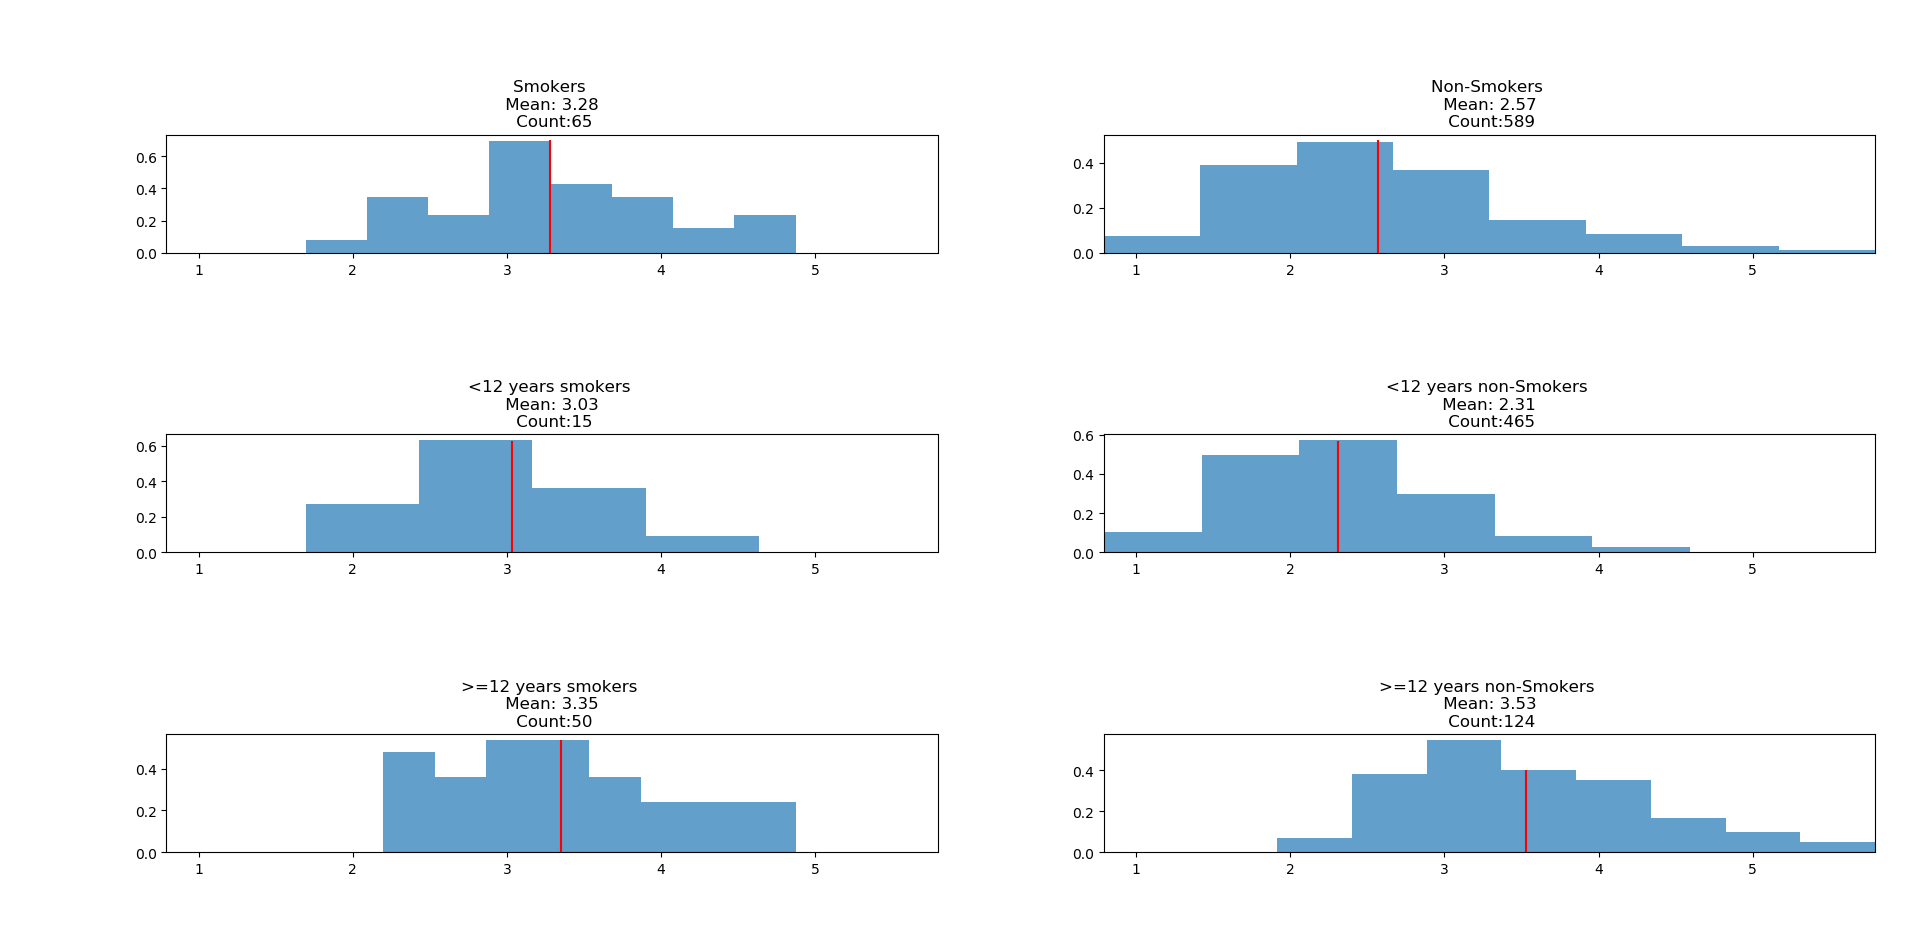
\includegraphics[width=150mm,height=115mm]{hist}	
\end{figure}

\end{appendix}

\end{document}
